\documentclass[12pt]{report}
\usepackage{verbatim}
\usepackage{fullpage}
\usepackage{etoolbox}
\usepackage{lipsum}
\usepackage{graphicx}
\usepackage{hyperref}
\usepackage{titlesec}
\usepackage{pdftexcmds}
\usepackage{minted}
\usepackage[utf8]{inputenc}


\graphicspath{ {res/} }
\setcounter{secnumdepth}{4}
\titleformat{\paragraph}
{\normalfont\normalsize\bfseries}{\theparagraph}{1em}{}
\titlespacing*{\paragraph}
{0pt}{3.25ex plus 1ex minus .2ex}{1.5ex plus .2ex}

\newcommand{\HRule}{\rule{\linewidth}{0.5mm}}
\renewcommand\emph{\textbf}
\renewcommand{\baselinestretch}{1.1}

\begin{document}
    \begin{titlepage}

        \center

        \textsc{\LARGE Universita' degli Studi di Messina}\\[0.1cm]
        \textsc{\Large Dipartimento di Matematica e Informatica}\\[0.5cm]
        \textsc{\Large Progetto Sistemi Operativi}\\[0.5cm]

        \HRule \\[0.4cm]
        { \huge \bfseries AllocSim}\\[0.1cm]

        {\large 24 June 2015}
        \HRule \\[1.5cm]

        \begin{minipage}{0.4\textwidth}
        \begin{flushleft} \large
        \emph{Author:}\\
        Vittorio \textsc{Romeo}
        \end{flushleft}
        \end{minipage}
        ~
        \begin{minipage}{0.4\textwidth}
        \begin{flushright} \large
        \emph{Professors:} \\
        Santa \textsc{Agreste}

        \end{flushright}
        \end{minipage}\\[4cm]

        \vfill

        \begin{minipage}{\linewidth}
            \centering
            \begin{minipage}{0.35\linewidth}
                \begin{figure}[H]
                    \center
                    
\includegraphics[width=2cm, height=2cm]{logovee}

                    \url{http://vittorioromeo.info}
                \end{figure}
            \end{minipage}
            \hspace{0.27\linewidth}
            \begin{minipage}{0.35\linewidth}
                \begin{figure}[H]
                    \center
                    
\includegraphics[width=2cm, height=2cm]{logounime}

                    \url{http://unime.it}
                \end{figure}
            \end{minipage}
        \end{minipage}\\[3cm]
    \end{titlepage}

    \pagenumbering{gobble}
    \newcommand{\atoc}[1]{\addtocontents{toc}{#1\par}}
    \renewcommand{\thesection}{\arabic{section}.}
    \tableofcontents
    \newpage
    \pagenumbering{arabic}

    \section{Richiesta}
        Si richiede l’implementazione di un applicativo che simuli tre delle tecniche usate per eseguire l’allocazione della memoria utilizzando una free-list: \emph{first-fit}, \emph{best-fit} e \emph{worst-fit}. 

        L’applicativo deve prevedere una situazione iniziale (randomica) della memoria e confrontare il risultato finale ottenuto dalle tre tecniche. 

        Supponendo che ogni confronto costi una unitò, si analizzino le differenze in termini di costo e in termini di frammentazione esterna.         

        L’applicativo deve effettuare delle simulazioni al fine di esaminare il diverso comportamento delle tre tecniche mostrando ad ogni simulazione lo stato del sistema sia a video che su file di log.

        L’applicativo deve essere sviluppato in \emph{Python}.

    \section{Design ed implementazione}
        L'architettura dell'applicazione è stata designata utilizzando \emph{principi OOP} (Object-Oriented Programming) e massimizzando la riusabilità delle classi.

        Nella lista seguente sono riportati gli elementi che compongono l'architettura e il modo in cui sono relazionati:

        \begin{itemize}
            \item \emph{Blocco di memoria}: classe Python \mintinline{python}{Block} - rappresenta porzione dell'area di memoria presente nell'\emph{Allocatore}. Può essere \emph{occupato} o \emph{libero}, ha un \emph{byte di inizio} ed un \emph{byte di fine}.
            \item \emph{Allocatore}: classe Python \mintinline{python}{Allocator} - rappresenta un'area di memoria contigua che può essere frammentata ed utilizzata per instanziare \emph{processi}. L'area di memoria viene divisa in \emph{blocchi}.  Contiene una lista di blocchi ordinata per posizione (in byte), una lista di blocchi ordinata per grandezza (utilizzata per implementare versioni degli algoritmi \emph{best-fit} e \emph{worst-fit} più efficienti), ed una lista di blocchi calcolata a runtime dei blocchi adiacenti liberi (\emph{boundary-tag}). 
            L'allocatore permette di \emph{dividere} un blocco in due in una specifica posizione, di \emph{occupare} o \emph{liberare} la memoria, e di \emph{unificare} i blocchi contigui liberi.
            L'allocatore contiene tutta la logica riguardante l'esecuzione degli \emph{algoritmi} richiesti, ed anche la logica per la generazione di un \emph{grafico ASCII} che rappresenta lo stato dell'area di memoria.
            \item \emph{Algorithmi}: contenuti nella classe Python \mintinline{python}{Allocator} - oltre agli algoritmi richiesti (\emph{first-fit}, \emph{best-fit}, \emph{worst-fit}), sono stati designati ed implementati anche i seguenti: \emph{next-fit}, \emph{best-fit} (con lista ordinata), e \emph{worst-fit} (con lista ordinata).
            Gli algoritmi agiscono sui \emph{blocchi}, liberi o occupati da \emph{processi}.
            \item \emph{Simulazione}: gestite da Python tramite le funzioni \mintinline{python}{runSimulations} and \mintinline{python}{simulate} - una simulazione, al suo inizio, genera una lista randomica di \emph{processi}, la quale viene testata in N \emph{sottosimulazioni}, le quali eseguono uno degli \emph{algoritmi} sulla medesima lista di processi, restituendo un \emph{set di risultati}.
            \item \emph{Sottosimulazione}: esegue un \emph{algoritmo} su un set di \emph{processi} generato randomicamente. Pulisce l'\emph{allocatore} dalle sottosimulazioni precedenti ed esegue calcoli statistici per verificare l'efficienza di un algoritmo, riportata in un \emph{set di risultati}.
            \item \emph{Processo}: classe Python \mintinline{python}{Process} - rappresenta un processo del sistema operativo utilizzato per le simulazioni automatiche. Ogni processo ha un \emph{tempo di entrata} (momento in cui il sistema prova ad allocare il processo), un \emph{tempo di esecuzione} (numero di unità di tempo necessarie al completamento del processo), un numero di \emph{byte richiesti} per l'esecuzione del processo (che saranno forniti, se possibile, attraverso l'allocazione di un \emph{blocco} libero). I processi randomicamente vengono generati all'inizio di una \emph{simulazione}.
            \item \emph{Set di risultati}: instanziato e stampato alla fine di una \emph{simulazione}. Contiene informazioni riguardo il \emph{numero di comparazioni}, \emph{frammentazione media} e \emph{punteggio totale} di ogni \emph{algoritmo} testato durante la simulazione. Minore il punteggio, più efficiente l'algoritmo.
        \end{itemize}

        L'applicativo può essere eseguito in due modalità: \emph{modalità manuale} e \emph{modalità automatica}.

        \begin{itemize}
            \item \emph{Modalità manuale}: gestita dalla funzione Python \mintinline{python}{mainManual} - questa modalità permette all'utente di interagire manualmente con l'\emph{allocatore}, eseguendo allocazioni singole e visualizzando tramite un \emph{grafico ASCII} il loro risultato.

            \item \emph{Modalità automatica}: gestita dalla funzione Python \mintinline{python}{mainAutomatica} - genera N simulazioni (valore passato da linea di comando, come primo parametro) e le esegue, scrivendo a video e su log i loro risultati. 
        \end{itemize}

    \section{Diagramma UML}
        Viene qui riportato il \emph{class diagram UML} delle classi contenute nel progetto.
        Il diagramma è stato realizzato automaticamente dall'applicazione \mintinline{python}{pyreverse}.

        \begin{figure}[H]
            \caption{Diagramma UML delle classi.}
            \centering
            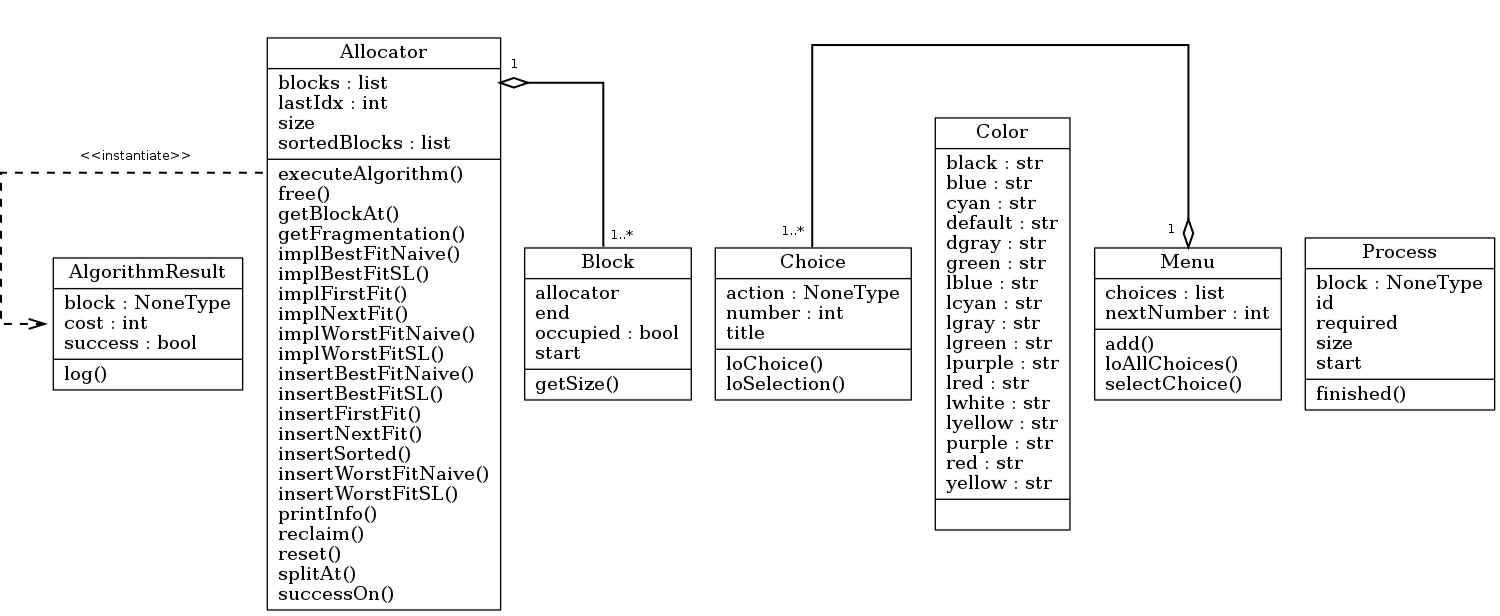
\includegraphics[width=1\textwidth]{diatemp}
        \end{figure}

    \section{Manuale d'uso}

        L'applicazione è molto \emph{user-friendly}: semplice da usare e robusta. Gli input forniti dall'utente vengono controllati, ed in caso di input non validi l'utente può ritentare senza causare errori o crash.

        \subsection{Modalità manuale}

            Per avviare l'applicazione in \emph{modalità manuale} è sufficiente lanciarla da linea di comando senza parametri:

            \begin{minted}[mathescape, linenos, numbersep=5pt, gobble=2, frame=lines, framesep=2mm, fontsize=\footnotesize]{bash}
                ./project.py
            \end{minted}

            Dopo aver avviato il programma, l'utente vedrà il seguente menù:

            \begin{figure}[H]
                \caption{Screenshot - menù modalità manuale.}
                \centering
                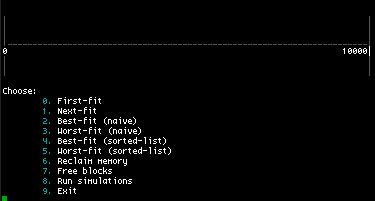
\includegraphics[width=0.8\textwidth]{scr1}
            \end{figure}

            L'utente potrà scegliere tra le varie funzioni dell'allocatore e visualizzare su schermo in maniera grafica i loro risultati.

        \subsection{Modalità automatica}

            Per avviare l'applicazione in \emph{modalità automatica} è sufficiente lanciarla da linea di comando con il numero di simulazioni desiderato:

            \begin{minted}[mathescape, linenos, numbersep=5pt, gobble=2, frame=lines, framesep=2mm, fontsize=\footnotesize]{bash}
                # Esempio (3 simulazioni) 
                ./project.py 3
            \end{minted}

            Dopo aver avviato il programma, le simulazioni partiranno automaticamente ed il loro funzionamento sarà mostrato sia a video che su log.

\end{document}
